\documentclass[a4paper, 12pt]{article}
\renewcommand{\baselinestretch}{1.22}

% Packages
\usepackage[T1]{fontenc}
\usepackage[utf8]{inputenc}
\usepackage[ngerman]{babel}
\usepackage[ngerman=ngerman-x-latest]{hyphsubst}

\usepackage[a4paper, inner=2.5cm, outer=2.5cm, top=2.5cm, bottom=2.5cm, bindingoffset=0cm]{geometry}
\usepackage{float}
\usepackage{csquotes}
\usepackage{graphicx}

\usepackage[citestyle=verbose-ibid,giveninits=true,doi=false,eprint=false,isbn=false,backend=biber]{biblatex}
\usepackage[bottom]{footmisc}
\addbibresource{bib/main.bib}
\DeclareNameAlias{default}{family-given}
\DeclareDelimFormat[bib]{nametitledelim}{\addcolon\space} % Doppelpunkt nach Autor

\graphicspath{{figures/}}

\begin{document}

\title{\vspace{-2.0cm}Surrealismus und Wahrnehmung\\\enquote{Der Therapeut}}
\author{Marvin Borner, Philosophie TG13}
\date{\today}

%{\parindent 0cm
%	\subsection*{Selbstständigkeitserklärung}
%	Ich erkläre hiermit, dass ich die vorliegende Arbeit selbstständig verfasst
%	und nur unter Verwendung der angegebenen Quellen und Hilfsmittel angefertigt habe.\\
%	\vspace{1\baselineskip}
%
%	Langenau, den \today \hspace{0.1\linewidth}
%}

\maketitle

\begin{figure}[H]
	\centering
	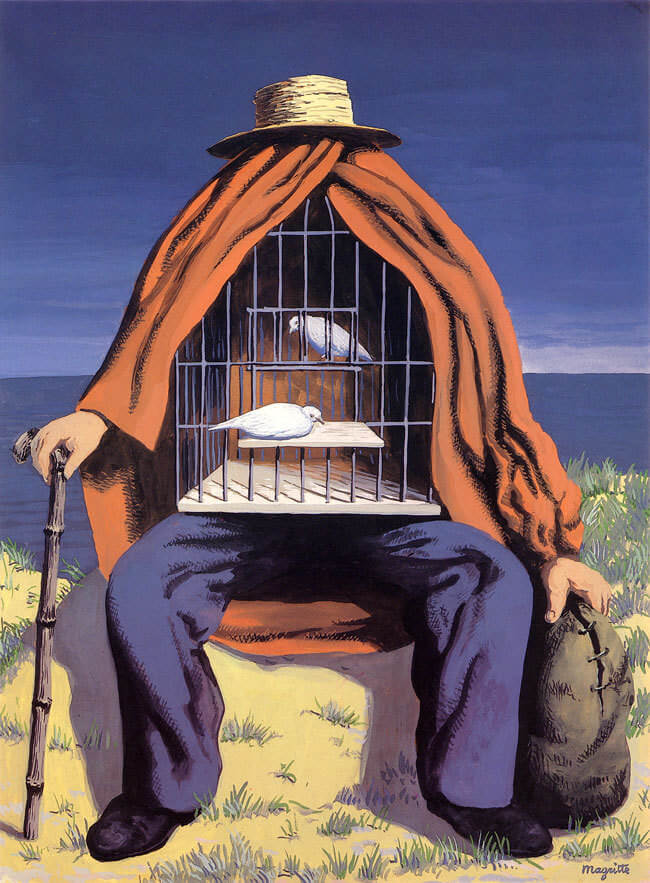
\includegraphics[height=9cm]{the-therapist}
	\caption{\enquote{Der Therapeut} (1937) von René Magritte $^1$}
\end{figure}

\section{Erstbetrachtung}
In dem Gemälde \enquote{Der Therapeut} (aus dem Englischen \enquote{The Therapist}), welches im Jahr 1937 von René Magritte gemalt wurde\footcite{therapist}, sieht man eine Person, die mit einem roten Umhang umhüllt am Strand auf einem Sandhügel vor einem Meer sitzt. Die Person hat allerdings einen Käfig mit weißen Tauben als Oberkörper und besitzt offensichtlich auch keinen Kopf, da der Hut direkt auf dem Käfig liegt. Der genannte Käfig scheint allerdings offen zu sein. Zudem hält die Person einen Gehstock in der rechten Hand. In der linken Hand hält die Person eine dunkle Tasche. Da diese Umstände nicht der Realität entsprechen, ist das Bild vom Surrealismus geprägt.

Schon bei dem ersten Anblick dieses Bildes kommen viele Fragen auf: Warum besitzt die Person keinen Oberkörper oder Kopf? Warum hat sie einen Umhang um? Was bedeuten die Tauben in dem Käfig? Warum bleiben die Tauben im offenen Käfig und fliegen nicht einfach weg? Was ist in der Tasche? Will die Person aufbrechen, entfliehen? Warum heißt das Gemälde \enquote{Der Therapeut}? Wer wird hier therapiert? Wir als Betrachter, die Person selbst, die Vögel, die gesamte Menschheit?

Möglicherweise sind es auch genau diese Fragen und die Gedanken, die durch die Versuche, diese zu beantworten, therapeutische Effekte in der betrachtenden Person hervorrufen sollen. Offensichtlich ist es aber, dass dieses Bild - wie so häufig bei surrealen Bildern - keine eindeutige Interpretation, sondern vielmehr eine subjektive Reise durch persönliche Erfahrungen und Assoziationen bietet.

\section{Reise}
Wie schon gesagt, verursacht der erste Eindruck des Bildes Irritation und Verwirrung im Betrachter. Die Kombination des roten Umhangs, den weißen Tauben und dem beinahe lilanem Blauton des Himmels, des Wassers und der Hose lassen das gesamte Bild mysteriös, beinahe magisch, wirken.

Da die Tauben im \textit{Innern} des Käfigs sind, welcher wiederum der Oberkörper der Person ist, kommt man schnell zu dem Schluss, dass die Tauben eine \textit{innere} Verbindung mit der Person haben müssen. Die Tauben könnten folglich für die Vorstellungskraft, Gedanken, Geheimnisse und Erfahrungen - den Geist? - stehen, welche die Person besitzt. Schließlich besizt die Person außer ihren Händen (beziehungsweise den nicht sichtbaren Armen) nur noch die Beine und Füße, was bedeutet, dass der Käfig - und somit die Tauben - einzig und allein für alles andere zuständig sein müssen.

Die Anzahl und die Position der Tauben könnte auch eine Versinnbildlichung des klassischen dualistischen Leib-Seele-Problems sein. Die physische Entität könnte demnach die obere Taube, also die Taube, die weiter im Körper der Person ist, sein, während die mentale Entität von der unteren Taube repräsentiert wird, welche eher an einem etwas offeneren Ort platziert ist und somit die offenen Fähigkeiten und die potentielle Stärke der Vorstellungskraft darstellt, welche mit den mentalen Fähigkeiten erreichbar sind. Dass die untere Taube, also die mentale Entität, nun nicht wegfliegt, könnte die Grenzen unserer Vorstellungskraft demonstrieren. \enquote{Über den Tellerrand hinaus} zu schauen, die \enquote{Komfortzone} zu verlassen und der Fantasie freien Lauf zu lassen, mag wohl eine der vielen Interpretationen des Sinnes dieses Bildes sein.

Diese Interpretation wird auch von der Darstellung des roten Umhangs unterstützt. Denn der Umhang behindert die Sicht der Tauben, so dass sie nur eine Seite der Umgebung sehen können. Zu bedenken ist auch, dass Umhänge normalerweise freiwillig angezogen werden und auch selbstständig wieder abgenommen werden können. Versinnbildlicht bedeutet dies, dass unsere Wahrnehmung, Vorstellungskraft und Fantasie - also die mentale Entität - durch uns selbst begrenzt wird und nur dadurch voll ausgenutzt werden kann, wenn wir unserer Fantasie freien Lauf lassen (ergo die Taube wegfliegt) oder unsere selbstgesetzten mentalen Grenzen ignorieren (ergo den Umhang abnehmen) beziehungsweise ausdehnen. Nur so ist es möglich, auch die andere Seite der Welt in vollem Umfang wahrzunehmen.

Wir als Menschen sind allzu oft derartig auf eine Denkrichtung fokussiert, dass es dazu kommen kann, die andere Richtung (vgl. das Meer) zu ignorieren oder zu vergessen. Sowohl in der Wissenschaft, als auch in der Politik und im allgemeinen Leben ist es also wichtig, seinen eigenen Umhang abzunehmen um eine zu starke einseitige Polarisierung zu vermeiden und alle Seiten zu beachten. Beispiele einer solchen Fokussierung sind die aktuellen Querdenker, die durch ihre gezielt begrenzten Denkrichtungen eine große Menge an jenen Personen mit Käfig und Umhang erschaffen haben, die sich als Verschwörung widersetzen, die andere Sichtweise in Betracht zu ziehen.

Auch der Wanderstock und die Tasche unterstützen diese Interpretation. Die \textit{sitzende} Person stellt hiermit den eigenen Unwillen dar, sich selbstständig in \textit{Bewegung} zu versetzen, aktiv nach anderen Sichtweisen Ausschau zu halten und die zuvor genannte subjektive vermeintliche Grenze der Vorstellungskraft zu überschreiten. Der Wanderstock und die Tasche könnte hier eine weitere Anspielung darauf sein, dass wir dazu selbst in der Lage sind und die Fähigkeiten und Voraussetzungen, unsere eigene Reise durch die Fantasie und Gedanken-/Lebens-Vielfalt zu unternehmen, bereits besitzen.

Zuletzt ist das Meer wohl noch ein zusätzlicher Hinweis auf die Schönheit der Diversität, die uns das Überschreiten unserer selbstgesetzten Grenzen erblicken lassen kann.

\section{Suche}
Das Interessante an diesem Gemälde ist, dass sich nach längerer Suche trotz anfänglicher Verwirrung ein Sinn und eine Interpretation bildet. Interessant deshalb, weil eben dieses Phänomen, über den Wahrnehmungshorizont hinaus zu denken und in die Tiefen des Bildes einzutauchen, sowohl die Suche beendet hat, als auch die eigentliche Bedeutung des Bildes ist.

Die Suche nach Sinn ist bei Menschen vorprogrammiert. Sowohl im Bezug zum Leben, als auch im Bezug zu allgemeinen Umständen und Gegebenheiten. Denn die ständigen Fragen, weshalb Dinge so sind, wie sie sind und weshalb sie sich dort befinden, wo sie sind, haben uns als Menschheit schließlich erst zu dem gemacht, wozu wir heutzutage sowohl technisch als auch wissenschaftlich in der Lage sind.

Unter normalen Umständen ist unsere Fantasie dann auch erstaunlich gut darin, nach einer kurzen Betrachtung nicht ganz offensichtlicher Umstände, den Sinn dahinter zu finden, Lücken der Wahrnehmung zu füllen und verdeckte oder manipulierte Objekte in ihre Ursprungsform zurückzubringen. Doch manchmal, wie auch in diesem Gemälde, kommt unsere Fantasie und Vorstellungskraft an ihre Grenzen. Zwar ist unsere Wahrnehmung gut genug, eine Person in diesem verwirrenden Chaos von verschiedenen Objekten zu sehen, ein größerer Sinn ist auf den ersten Blick allerdings nicht zu erkennen.

Derartige Manifestationen von surrealen Objekten lösen trotz der anfänglichen Verwirrung dennoch eine Neugierde aus, die einen Betrachter nahezu fesseln kann und diesen somit quasi dazu zwingt, die vermeintlichen Grenzen dessen Fantasie zu durchbrechen. René Magritte sagt passend dazu in einem Kommentar zu seinem populären Gemälde \enquote{Der Sohn des Mannes}: \enquote{Es gibt ein Interesse an dem, was verborgen ist und was das Sichtbare uns nicht zeigt. Dieses Interesse kann die Form eines recht intensiven Gefühls annehmen, eine Art Konflikt könnte man sagen \textelp{}}\footcite{sonofman}. Eben dies ist der Grund für all die optischen Täuschungen und surrealen Bilder, deren einziger Sinn häufig die Verwirrung und der daraus entstehende Gedankenspaziergang durch mögliche Erklärungen und die darauffolgende persönliche Entfaltung und die Erkenntnis, dass nicht alles, was wir sehen, so ist, wie es im ersten Moment scheint, die Grenzen der Fähigkeiten unserer Fantasie dehnbar sind und unsere initiale Wahrnehmung inkorrekt sein kann, ist.

%\newpage
%
%\nocite{*}
%\printbibliography[heading=bibintoc]

\end{document}
